Redux es un administrador de estado predecible para aplicaciones JavaScript basado en el patrón de diseño Flux. A medida que una aplicación crece, se hace difícil mantenerla organizada y mantener el flujo de datos. Redux resuelve este problema administrando el estado de la aplicación con un único objeto global llamado Redux Store. Los principios fundamentales de Redux ayudan a mantener la coherencia en toda la aplicación, lo que facilita la depuración y las pruebas.

\subsubsection{Redux/Flux}
Redux adoptó un gran número de restricciones de la arquitectura Flux: las acciones encapsulan la información para que el Redux Reducer actualice el estado de manera determinista, el estado es un Redux Store singleton. El despachador de Flux único se reemplaza con múltiples Redux Reducers pequeños que recogen información de las acciones y la `reducen' a un nuevo estado que luego se guarda en lel Redux Store. Cuando se cambia el estado en el Store, la Vista según la suscripción recibe propiedades.

\begin{figure}[H]
  \centering
  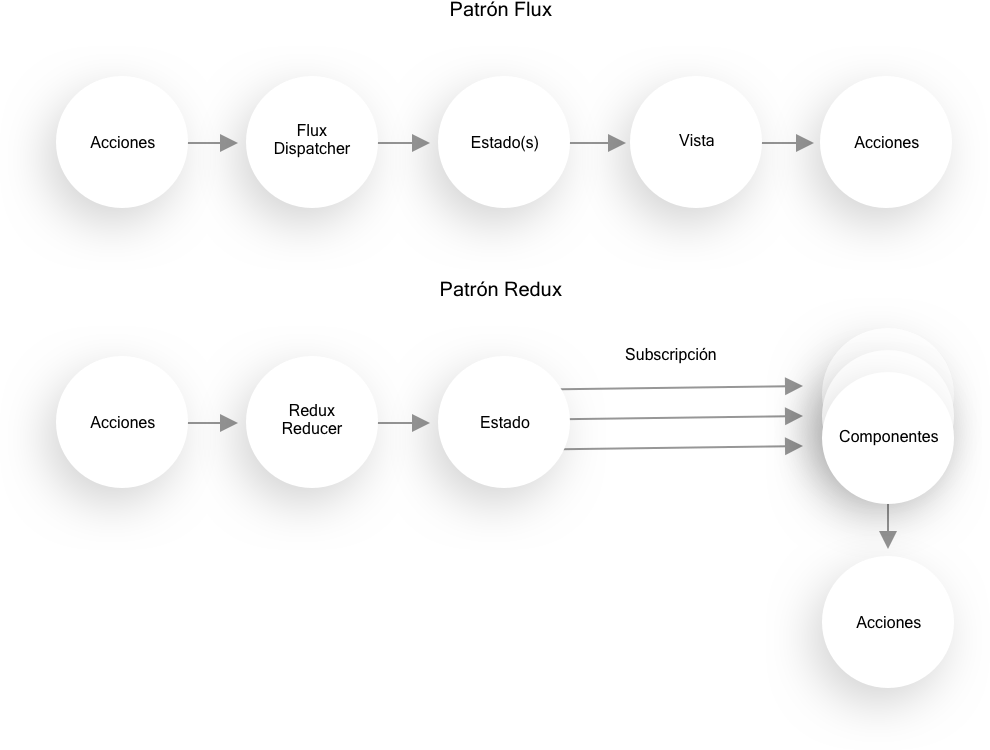
\includegraphics[width=0.9\textwidth]{flux-redux}
  \caption{Comparación Flux/Redux.}
\end{figure}

\subsubsection{Redux Store}
Redux Store contiene un objeto del estado global de la aplicación. Esta actualiza el estado y notifica los componentes suscritos.
\vspace{0.8cm}

\lstinputlisting[style=ES6, caption=Fragmento de código para inicializar el Redux Store]{code/redux-store.js}

\subsubsection{Redux Reducer}
Un Redux Reducer es solo una función pura de JavaScript. Recibe dos parámetros: el estado actual y la acción. Una función pura es aquella que devuelve exactamente la misma salida para la entrada dada. El estado es el objeto Redux Store completo, la acción es el objeto despachado con un tipo requerido y un payload opcional.
\vspace{0.8cm}

\lstinputlisting[style=ES6, caption=Fragmento de código del reducer común de la app]{code/redux-reducer.js}

\subsubsection{Acciones Redux}
La única forma de cambiar el estado es enviando una señal a el Store. Esta señal es una acción. Entonces "despachar una acción" significa enviar una señal a el Redux Store.
\vspace{0.8cm}

\lstinputlisting[style=ES6, caption=Fragmento de código de la acción que valida a un administrador]{code/redux-action.js}
